\documentclass{beamer}

\usepackage{palatino}
\usepackage{amsfonts}
\usepackage{fancyvrb}
\usepackage{graphicx}
\usepackage{url}
\usepackage[utf8]{inputenc}
%\usepackage[all]{xypic}

% To show source
\DefineVerbatimEnvironment{source}{Verbatim}%
{commandchars=\\\{\}}

\DefineVerbatimEnvironment{sourcex}{Verbatim}%
{fontsize=\footnotesize,commandchars=\\\{\}}

% Sets
\newcommand{\set}[1]{\{#1\}}
\newcommand{\such}{\mid}
\newcommand{\pair}[1]{\langle #1 \rangle}
\newcommand{\prop}{\Sigma}

% Common sets
\newcommand{\NN}{\mathbb{N}}
\newcommand{\ZZ}{\mathbb{Z}}
\newcommand{\QQ}{\mathbb{Q}}
\newcommand{\RR}{\mathbb{R}}

\newcommand{\RRasc}{\underline{\RR}}
\newcommand{\RRdesc}{\overline{\RR}}

% Quantifiers
\newcommand{\all}[3]{\forall\, #1 \,{\in}\, #2\,.\left(#3\right)}
\newcommand{\some}[3]{\exists\, #1 \,{\in}\, #2\,.\left(#3\right)}
\newcommand{\xall}[3]{\forall\, #1 \,{\in}\, #2\,.\,#3}
\newcommand{\xuall}[2]{\forall\, #1 \,.\,#2}
\newcommand{\uall}[2]{\forall\, #1 \,.\,\left(#2\right)}
\newcommand{\usome}[2]{\exists\, #1 \,.\,\left(#2\right)}
\newcommand{\xsome}[3]{\exists\, #1 \,{\in}\, #2\,.\,#3}
\newcommand{\xusome}[2]{\exists\, #1 \,.\,#2}

\newcommand{\cut}[3]{\mathsf{cut}\; #1\; \mathsf{left}\ #2\ 
  \mathsf{right}\  #3}

\newcommand{\xcut}[3]{\begin{aligned}[t]
\mathsf{cut}\; #1 \ \ \mathsf{left}\  &#2 \\
\mathsf{right}\ &#3 
\end{aligned}}

\title{Programming Techniques for\\
Exact Real Arithmetic}
\author{Andrej Bauer\\
{\footnotesize Faculty of Mathematics and Physics}\\
{\footnotesize University of Ljubljana, Slovenia}\\[2ex]
(joint work with Ivo List \& Paul Taylor)
}
\date{SCAN 2014, Würzburg, September 2014}

\beamerdefaultoverlayspecification{<+->}
\mode<presentation>
% \usetheme{Goettingen}
\usecolortheme{rose}
\usefonttheme{serif}
\setbeamertemplate{navigation symbols}{}

% Frame number
\setbeamertemplate{footline}[frame number]{}

\begin{document}

\begin{frame}
  \titlepage
\end{frame}

\begin{frame}
  \frametitle{In this talk}

  \begin{quote}
    We present a mathematical language \textbf{Marshall} which is powerful enough to
    let us talk about real analysis, but also simple enough to be an efficient programming
    language.
  \end{quote}


  \pause

  \begin{itemize}
  \item \emph{Descriptive} language -- \emph{what} to compute.
  \item \emph{How} to compute?
    %
    \begin{itemize}
    \item We present a simple-minded execution strategy
    \item Many possibilities for optimization
    \end{itemize}
  \item Applications:
    %
    \begin{itemize}
    \item specification of computational problems
    \item verification of safety and liveness properties
    \end{itemize}
  \end{itemize}
\end{frame}

\begin{frame}
  \frametitle{Foundations: Abstract Stone Duality}

  \begin{itemize}
  \item Our language is based on \emph{Abstract Stone
      Duality} (ASD) by Paul Taylor.
  \item ASD is a variant of $\lambda$-calculus which directly
    axiomatizes spaces and continuous maps.
  \item We use a fragment of ASD which can be understood on its own.
  \item Further material: \url{http://www.paultaylor.eu/ASD/}
  \end{itemize}

\end{frame}

\begin{frame}
  \frametitle{Axioms for real numbers}

  The real numbers $\RR$ are:
  %
  \begin{itemize}
  \item an ordered field (``can compute with reals'')
  \item with Archimedean property (``can obtain approximations'')
  \item Dedekind complete (``can use iterative methods'')
  \item overt Hausdorff space (``can search for a witness'')
  \item and $[a,b]$ is compact (``can verify something holds'')
  \end{itemize}
\end{frame}

\begin{frame}
  \frametitle{Dedekind cuts}

  A \emph{cut} is a pair of \emph{rounded}, \emph{bounded},
  \emph{disjoint}, and \emph{located} open sets.

  \bigskip

  \begin{center}
    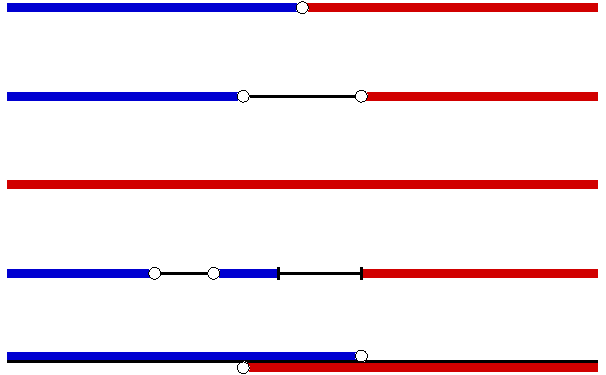
\includegraphics[width=0.75\textwidth]{cuts}
  \end{center}

\end{frame}

\begin{frame}
  \frametitle{Lower and upper reals}

  By taking the lower rounded sets we obtain the \emph{lower reals},
  and similarly for \emph{upper reals.} These are more fundamental
  than reals.

  \bigskip\bigskip

  \begin{center}
    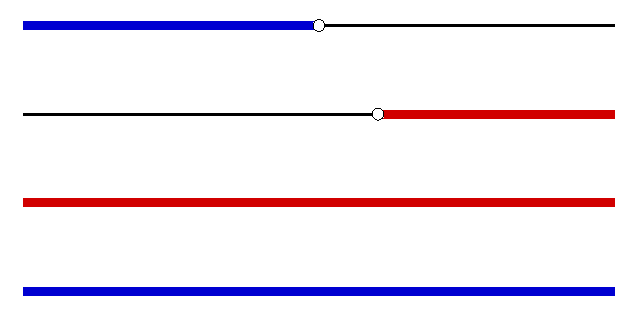
\includegraphics[width=0.75\textwidth]{lower_upper}
  \end{center}

\end{frame}

\begin{frame}
  \frametitle{Examples of cuts}

  \begin{itemize}

  \item A number $a$ determines a cut, which determines $a$:
    %
    \begin{equation*}
      a = (\cut{x}{x < a}{a < x})
    \end{equation*}
  \item $\sqrt{a}$ is the cut
    %
    \begin{equation*}
      \cut{x}{(x < 0 \lor x^2 < a)}{(x > 0 \land x^2 > a)}
    \end{equation*}
  \item Exercise:
    %
    \begin{equation*}
      \cut{x}{(x < -a \lor x < a)}{(-a < x \land a < x)}
    \end{equation*}
  \item The full notation for cuts is
    %
    \begin{equation*}
      \cut{x : [a,b]}{\phi(x)}{\psi(x)}
    \end{equation*}
    %
    This means that the cut determines a number in $[a,b]$.
  \end{itemize}

\end{frame}

\begin{frame}
  \frametitle{A language for real analysis}

  \begin{itemize}
  \item Number types $\NN$, $\QQ$, $\RR$
  \item Arithmetic $+$, $-$, $\times$, $/$
  \item Decidable equality $=$ and decidable order $<$ on $\NN$ and $\QQ$
  \item General recursion on $\NN$
  \item Semidecidable order relation $<$ on $\RR$
  \item Logic:
    \begin{itemize}
    \item truth $\top$ and falsehood $\bot$
    \item connectives $\land$ and $\lor$
    \item existential quantifiers:
      %
      \begin{equation*}
        \exists x : \RR, \quad
        \exists x : [a,b], \quad
        \exists x : (a,b), \quad
        \exists n : \NN, \quad
        \exists q : \QQ        
      \end{equation*}
    \item universal quantifier: \quad $\forall x : [a,b]$
    \end{itemize}
  \end{itemize}
\end{frame}

\begin{frame}
  \frametitle{``Topologic''}

  \begin{itemize}
  \item 
    A logical formula $\phi(x)$ where $x \in A$ has two readings:
    % 
    \begin{itemize}
    \item \emph{logical}: a predicate on $A$
    \item \emph{topological}:
      \begin{itemize}
      \item an open subset of $A$: $\phi(x) \iff \top$
      \item a closed subset of $A$: $\phi(x) \iff \bot$
      \end{itemize}
    \end{itemize}
  \item 
    In particular, a formula $\phi$ without parameters is
    % 
    \begin{itemize}
    \item \emph{logically}, a truth value
    \item \emph{topologically}, an element of Sierpinski space $\prop = \{\bot, \top\}$
    \end{itemize}
  \item 
    We use this to express topological and analytic notions
    \emph{logically}.
  \end{itemize}
\end{frame}

\begin{frame}
  \frametitle{Example: $\RR$ is locally compact}  

  \begin{itemize}
  \item Classically: for open $U \subseteq \RR$ and $x
    \in \RR$,
    %
    \begin{equation*}
      x \in U \iff \xsome{d,u}{\QQ}{x \in (d,u) \subseteq [d,u]
        \subseteq U}
    \end{equation*}

  \item Topologically: for $\phi : \RR \to \prop$ and $x : \RR$,
    %
    \begin{equation*}
      \phi(x) \iff
      \xsome{d,u}{\QQ}{d < x < u \land \xall{y}{[d,u]}{\phi(y)}}
    \end{equation*}
  \end{itemize}
\end{frame}

\begin{frame}
  \frametitle{Example: $[0,1]$ is connected}

  \begin{itemize}
  \item Classically: for open $U, V \subseteq [0,1]$, if
    %
    \begin{equation*}
      U \cap V = \emptyset \quad\text{and}\quad U \cup V = [0,1] 
    \end{equation*}
    then $U = [0,1]$ or $V = [0,1]$.
    %
  \item Topologically: for $\phi, \psi : [0,1] \to \prop$, if
    %
    \begin{align*}
      (\xsome{x}{[0,1]}{\phi(x) \land \psi(x)}) &\iff \bot \quad\text{and}\\
      (\xall{x}{[0,1]}{\phi(x) \lor \psi(x)}) &\iff \top
    \end{align*}
    then $(\xall{x}{[0,1]}{\phi(x)}) \lor (\xall{x}{[0,1]}{\psi(x)})$.
  \end{itemize}
\end{frame}

\begin{frame}
  \frametitle{$\forall\exists$ statements}

  {\LARGE
  \begin{equation*}
    \xall{x}{A}{\xsome{y}{B}{\phi(x,y)}}
  \end{equation*}}

  \pause

  \begin{itemize}
  \item ``For every parameter $x$ there is solution $y$.''
  \item ``In every state $x$ good thing $y$ happens.''
  \item Note: $A$ must be \emph{overt} and $B$ \emph{compact}.
  \end{itemize}
\end{frame}

\begin{frame}
  \frametitle{The maximum of $f : [0,1] \to \RR$}

    \begin{center}
      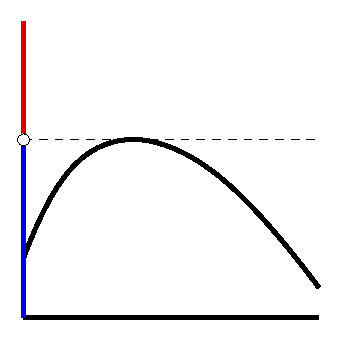
\includegraphics[width=0.5\textwidth]{max}
    \end{center}

    \begin{equation*}
      \xcut{x}{(\xsome{y}{[0,1]}{x < f(y)})}{(\xall{z}{[0,1]}{f(z) < x})}
    \end{equation*}
\end{frame}

\begin{frame}
  \frametitle{Cauchy completeness}

  \begin{itemize}
  \item A \emph{rapid} Cauchy sequence $(a_n)_n$ satisfies
    %
    \begin{equation*}
      |a_{n+1} - a_n| < 2^{-n}.
    \end{equation*}
    %
  \item Its limit is the cut
    % 
    \begin{equation*}
      \xcut{x}{(\xsome{n}{\NN}{x < a_n - 2^{-n+1}})}{(\xsome{n}{\NN}{a_n
          + 2^{-n+1} < x})}
    \end{equation*}
  \end{itemize}

\end{frame}

\begin{frame}
  \frametitle{From mathematics to programming}

  \begin{itemize}
  \item We would like to \emph{compute} with our language.
  \item We limit attention to logic and $\RR$.
  \item Not surprisingly, we compute with (improper) intervals.
  \end{itemize}
\end{frame}

\begin{frame}
  \frametitle{The interval lattice $L$}

  \begin{itemize}
  \item The lattice of \textbf{pairs} $[a,b]$, where $a$ is \emph{upper} and
    $b$ \emph{lower real}.
  \item Ordered by
    $[a,b] \sqsubseteq [c,d] \iff a \leq c \land d \leq b$.
  \item The lattice contains $\RR$ as $[a,a]$.
  \end{itemize}


  \begin{center}
    \input{interval_lattice.pdf_t}
  \end{center}
\end{frame}

\begin{frame}
  \frametitle{Extending arithmetic to $L$}

  \begin{itemize}\item 
    Extend operations from $\RR \times \RR \to \RR$ to $L \times L \to L$:
    %
    \begin{itemize}
    \item $L$ is equipped with the Scott topology
    \item \emph{any} continuous extension is acceptable
    \item (improper) intervals are understood \emph{order-theoretically}
    \end{itemize}
  \item The interesting case is \emph{Kaucher multiplication}.
  \item Given an arithmetical expression $e$ we compute its
    \emph{lower} and \emph{upper} approximants $e^{-}$ and $e^{+}$
    in~$L$:
    %
    \begin{equation*}
      e^{-} \sqsubseteq e \sqsubseteq e^{+}.
    \end{equation*}
    %
  \item
    We also extend $<$ to $L \times L \to \prop$:
    %
    \begin{equation*}
      [a,b] < [c,d] \iff b < c
    \end{equation*}
  \end{itemize}
\end{frame}

\begin{frame}
  \frametitle{Lower and upper approximants}

  \begin{itemize}
  \item For each sentence $\phi$ we define a \emph{lower} and
    \emph{upper approximants} $\phi^{-}, \phi^{+} \in \set{\top,
      \bot}$ such that
    %
    \begin{equation*}
      \phi^{-} \implies \phi \implies \phi^{+}.
    \end{equation*}
    %
  \item The approximants should be easy to compute.
  \item If $\phi^{-} = \top$ then $\phi = \top$, and if $\phi^{+} = \bot$ then $\phi = \bot$.
  \item Easy cases:
    %
    \begin{xalignat*}{2}
      \bot^{-} &= \bot
      &
      \bot^{+} &= \bot \\
      \top^{-} &= \top
      &
      \top^{+} &= \top \\
      (\phi \land \psi)^{-} &= \phi^{-} \land \psi^{-}
      &
      (\phi \land \psi)^{+} &= \phi^{+} \land \psi^{+}
      \\
      (\phi \lor \psi)^{-} &= \phi^{-} \lor \psi^{-}
      &
      (\phi \lor \psi)^{+} &= \phi^{+} \lor \psi^{+}
      \\
      (e_1 < e_2)^{-} &= (e_1^{-} < e_2^{-}) &
      (e_1 < e_2)^{+} &= (e_1^{+} < e_2^{+}).
    \end{xalignat*}
  \end{itemize}

\end{frame}

\begin{frame}
  \frametitle{Approximants for cuts and quantifiers}

  \begin{itemize}
  \item Cuts:
    %
    \begin{align*}
      (\cut{x : [a,b]}{\phi(x)}{\psi(x)})^{-} &= [a,b] \\
      (\cut{x : [a,b]}{\phi(x)}{\psi(x)})^{+} &= [b,a]
    \end{align*}
  \item Quantifiers:
    \begin{xalignat*}{5}
      &\phi([a,b])& &\implies& &\xall{x}{[a,b]}{\phi(x)}&
      &\implies& &\phi(\tfrac{a+b}{2}) \\
      \\
      &\phi(\tfrac{a+b}{2})& &\implies& &\xsome{x}{[a,b]}{\phi(x)}&
      &\implies& &\phi([b,a])
    \end{xalignat*}
  \end{itemize}
\end{frame}

\begin{frame}
  \frametitle{Refinement}

  \begin{equation*}
    \phi^{-} \implies \phi \implies \phi^{+}
  \end{equation*}
  
  \bigskip

  \begin{itemize}
  \item If $\phi^{-} = \bot$ and $\phi^{+} = \top$ we cannot
    say much about~$\phi$.
  \item To make progress, we \emph{refine} $\phi$ to an equivalent
    formula in which quantifers range over smaller intervals.
  \item A simple strategy is to split quantified intervals in halves:
    \begin{itemize}
    \item $\xall{x}{[a,b]}{\phi(x)}$ is refined to
      % 
      \begin{equation*}
        (\xall{x}{[a,\tfrac{a+b}{2}]}{\phi(x)}) \land
        (\xall{x}{[\tfrac{a+b}{2},b]}{\phi(x)})
      \end{equation*}
    \item $\xsome{x}{[a,b]}{\phi(x)}$ is refined to
      % 
      \begin{equation*}
        (\xsome{x}{[a,\tfrac{a+b}{2}]}{\phi(x)}) \lor
        (\xsome{x}{[\tfrac{a+b}{2},b]}{\phi(x)})
      \end{equation*}
    \end{itemize}
  \item This amounts to searching with \emph{bisection}.
  \end{itemize}
\end{frame}

\begin{frame}
  \frametitle{Refinement of cuts}

  \begin{itemize}\item 
    To refine a cut
    % 
    \begin{equation*}
      \cut{x : [a,b]}{\phi(x)}{\psi(x)}
    \end{equation*}
    % 
    we try to move $a \mapsto a'$ and $b \mapsto b'$.
    %
    \bigskip
    \begin{center}
      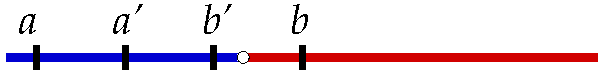
\includegraphics[width=0.7\textwidth]{cut_refine}
    \end{center}
    \bigskip
  \item 
    If $\phi^{-}(a') = \top$ then move $a \mapsto a'$.
  \item 
    If $\psi^{-}(b') = \top$ then move $b \mapsto b'$.
  \item One or the other endpoint moves eventually because cuts are
    located.
  \end{itemize}

\end{frame}


\begin{frame}
  \frametitle{Evaluation}

  \begin{itemize}
  \item To evaluate a sentence $\phi$:
    %
    \begin{itemize}
    \item if $\phi^{-} = \top$ then output $\top$,
    \item if $\phi^{+} = \bot$ then output $\bot$,
    \item otherwise refine $\phi$ and repeat.
    \end{itemize}
  \item Evaluation may not terminate, but this is expected, as $\phi$
    is only \emph{semi}decidable.
  \end{itemize}
\end{frame}

\begin{frame}
  \frametitle{Speeding up the computation}

  Estimate an inequality $f(x) < 0$ on $[a,b]$ by approximating $f$
  with a linear map from above and below.

  \begin{center}
    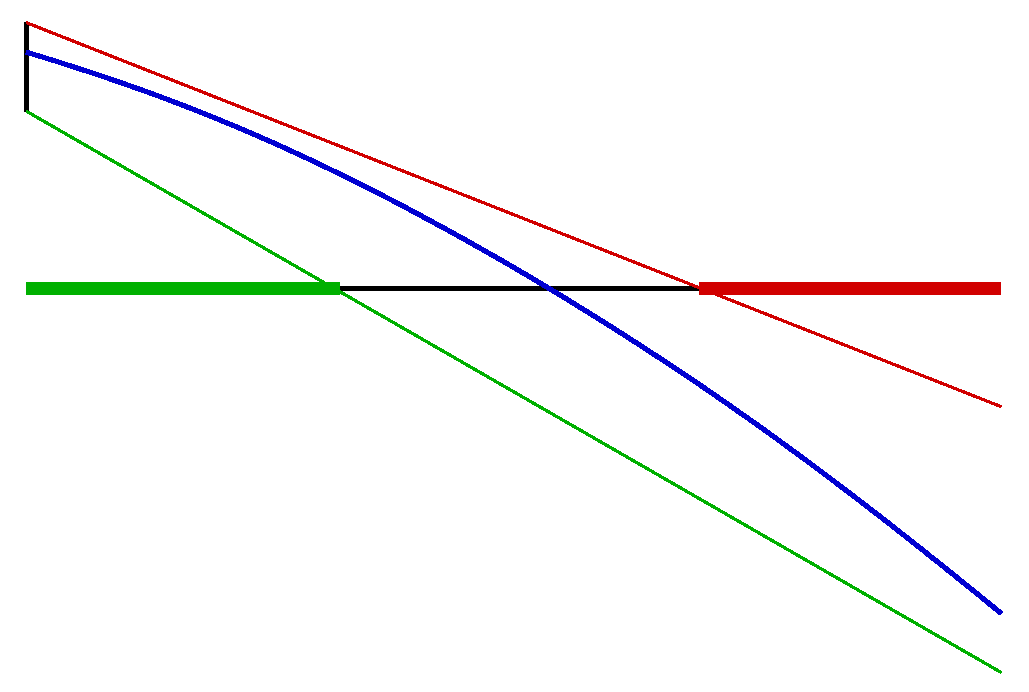
\includegraphics[width=0.7\textwidth]{newton}
  \end{center}

  This is essentially Newton's interval method.

\end{frame}

\begin{frame}
  \frametitle{Questions}

  \begin{itemize}
  \item How do we incorporate $\NN$ and recursion?
  \item How to extend Newton's method to improper intervals?
  \item How to extend Newton's method to the multivariate case?
  \item Can we do higher-type computations $\int$ and $\frac{d}{dx}$?
  \item Can this lead to a useful domain-specific language?
  \end{itemize}
\end{frame}

\end{document}
